\documentclass{article}

\usepackage[T1,T2A]{fontenc}
\usepackage[utf8]{inputenc}
\usepackage[english]{babel}
\usepackage{xcolor}
\usepackage{booktabs}
\usepackage{amsfonts}
\usepackage{algorithm}
\usepackage{algorithmicx}
\usepackage{algpseudocode}
\usepackage{amstext}
\usepackage{hyperref}
\usepackage{amssymb}
\usepackage{amsmath}
\usepackage{chemfig}
\usepackage{wrapfig}
\usepackage{subcaption}
\usepackage{tikz}
\usepackage{pgfplots}
\pgfplotsset{compat=1.18}

\usetikzlibrary{trees}

\bibliographystyle{apalike}

% aliases
\newcommand{\F}{\mathcal{F}}
\newcommand{\M}{\mathcal{M}}
\newcommand{\T}{\mathbb{T}}

\DeclareMathOperator*{\argmax}{arg\,max}
\DeclareMathOperator*{\argmin}{arg\,min}

\title{Substructure search optimizations}

\begin{document}
\maketitle

%\input{Introduction}
\input{introduction-fb}
\begin{figure}
\centering

\resizebox{!}{0.8\totalheight}	
{
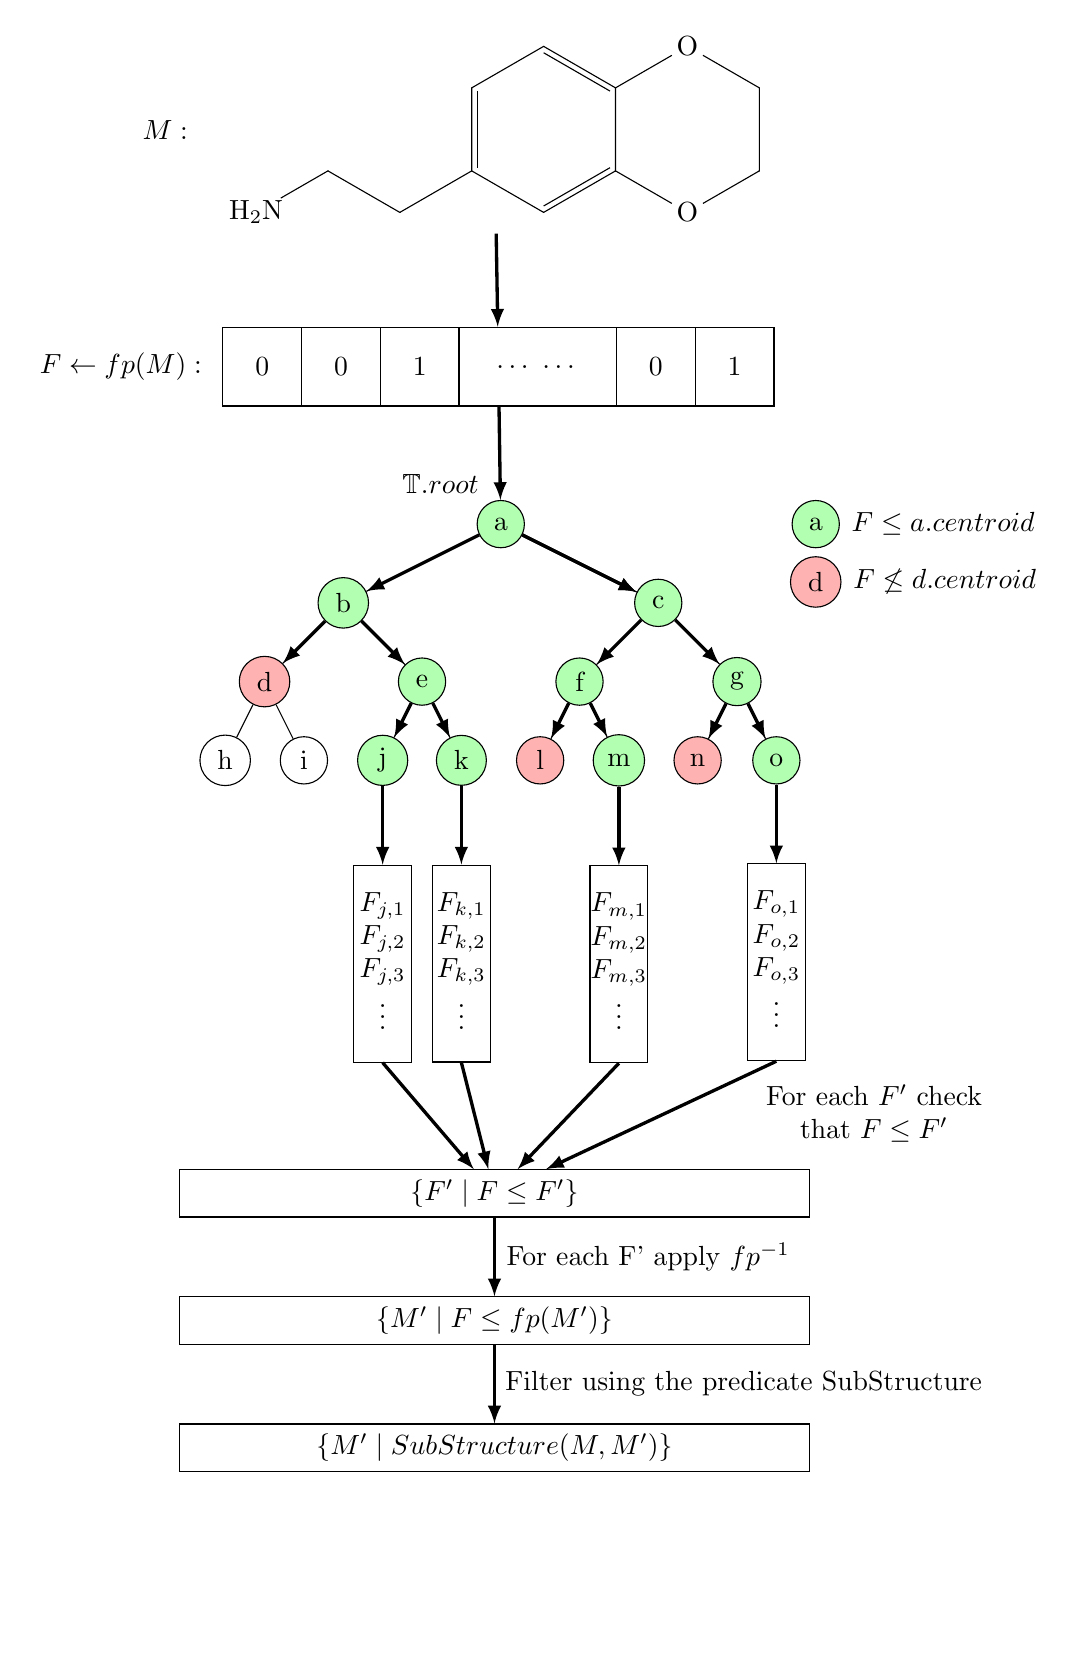
\begin{tikzpicture}[level distance=1cm,
  level 1/.style={sibling distance=4cm},
  level 2/.style={sibling distance=2cm},
  level 3/.style={sibling distance=1cm},
  every node/.style={circle,draw,minimum size=.6cm},
  bucket/.style={draw,rectangle,minimum height=2.5cm, text width=.5cm,align=center},
  stop_node/.style={fill=red!30},
  continue_node/.style={fill=green!30},
  arrow/.style={-latex,very thick},
  text_box/.style={rectangle,minimum width=8cm},
  fp_cell/.style={rectangle,draw,minimum width=1cm,minimum height=1cm},
  ]
  \usetikzlibrary{positioning}

  % molecule
  \node[name=molecule,rectangle,draw=none, minimum width=8cm]
  {
    \chemfig[angle increment=30,bond join=true]{
	*6(
	(
	-[-5]-[5]-
	{H_2N}
	)
	-=
	*6(
	-
	O
	---
	O
	-
	)
	-=-=
	)
    } 
  };

  % fingerprint
  \begin{scope}[yshift=-3cm,xshift=-2.95cm, minimum width=8cm]
    \node(fingerprint)[fp_cell,draw=none] at (3, 0) {};
    \node[fp_cell] at (0,0) {0};
    \node[fp_cell] at (1,0) {0};
    \node[fp_cell] at (2,0) {1};
    \node[fp_cell,minimum width=3cm] at (4,0) {  };
    \node[draw=none] at (3.5,0) {$\dots \ \dots$};
    \node[fp_cell] at (5,0) {0};
    \node[fp_cell] at (6,0) {1};
  \end{scope}

  % tree
  \begin{scope}[yshift=-5cm,xshift=0.08cm]
    \node[name=a,continue_node,label=170:{$\T.root$}] {a}
    child {node[name=b,continue_node]  {b}
      child {node[name=d,stop_node] {d}
	child {node[name=h] {h}}
	child {node[name=i] {i}}
      }
      child {node[name=e,continue_node] {e}
	child {node[name=j,continue_node] {j}}
	child {node[name=k,continue_node] {k}}
      }
    }
    child {node[name=c,continue_node] {c}
      child {node[name=f,continue_node] {f}
	child {node[name=l,stop_node] {l}}
	child {node[name=m,continue_node] {m}}
      }
      child {node[name=g,continue_node] {g}
	child {node[name=n,stop_node] {n}}
	child {node[name=o,continue_node] {o}}
      }
    };

    \begin{scope}[xshift=4cm,node distance=.1cm]
      \node (legend_a) [continue_node,label=right:{$F \le a.centroid$}] {a}; 
      \node (legend_d) [stop_node,below=of legend_a,label=right:{$F \not\le d.centroid$}] {d}; 
    \end{scope}
   
    \foreach \i in {j, k, m, o} {
      \node[name=bucket_\i,bucket,below=of \i]  {};
      \node[draw=none] at (bucket_\i.center) {
	  \begin{tabular}{c}
	    $F_{\i,1}$ \\
	    $F_{\i,2}$ \\
	    $F_{\i,3}$ \\
	    $\vdots$ 
	  \end{tabular} 
	};
    }
  \end{scope}
 
  % text boxes
  \begin{scope}[yshift=-13.5cm,node distance=1cm] 
    \node (filtered_fingerprints) [text_box]
      {
	$\{F' \mid F \le F'\}$ 
      };

  \foreach \i in {bucket_j, bucket_k, bucket_m}
    \draw[arrow] (\i.south) -- (filtered_fingerprints);


  \node (compounds) [text_box,below=of filtered_fingerprints]
    {
      $\{M' \mid F \le fp(M')\}$ 
    };
  
  \node (filtered_compounds) [text_box,below=of compounds]
    {
      $\{M' \mid SubStructure(M, M')\}$ 
    };
  \end{scope}

  % Arrows 
  \draw[arrow] (molecule) -- (fingerprint);
  \draw[arrow] (fingerprint) -- (a);  
  \foreach \from/\to in {a/b, b/d, e/j, c/f, f/l, g/n, a/c, b/e, e/k, a/c, c/g, g/o, f/m}
    \draw[arrow] (\from) -- (\to);

  \foreach \from/\to in {j/bucket_j, k/bucket_k, m/bucket_m, o/bucket_o}
    \draw[arrow] (\from) -- (\to);
  \draw[arrow] (bucket_o.south) -- (filtered_fingerprints) 
    node[draw=none,right,midway,xshift=9mm] 
    {
      \begin{tabular}{c}
	For each $F'$ check \\
	that $F \le F'$ 
      \end{tabular}
    };

  \draw[arrow] (filtered_fingerprints) -- (compounds)
    node[draw=none,right,midway]
    {
      For each F' apply $fp^{-1}$ 
    };

  \draw[arrow] (compounds) -- (filtered_compounds)
    node[draw=none,right,midway]
    {
      Filter using the predicate SubStructure 
    };
  
  % Labels
  \node[left=of molecule,draw=none,xshift=1.3cm] {$M:$}; 
  \node[left=of fingerprint,draw=none,xshift=-2.1cm] {$F \gets fp(M):$}; 

\end{tikzpicture}
}
\end{figure}

\section{Algorithm description}

\subsection{Notation}

The objective of the search is primarily to identify specific substructures within the molecules present in the 
given database $\M$.

To facilitate this search, we employ the concept of a ``fingerprint'', i.e. a binary string of a constant length 
${\sf fl}$ corresponding to every molecule. We can perform a fingerprint using a function ${\sf fp}: \M \to \F$, 
where $\F = \{{\sf fp}(M) \mid M \in \M\}$. This function takes a molecule from the set $\M$ and returns a binary 
string, the fingerprint in the set $\F$. Each fingerprint $F$ has bits  $F[i]$ for $i\in\{ 1,\ldots, {\sf fl}\}$.

To optimize the search process within the database $\M$, we aim to organize these fingerprints $\F$ in a 
structured manner. We propose the construction of a binary search tree, denoted as $\T$. Each node $\tt{v}$ 
in the tree $\T$ holds a set $\tt{v.set}$ of fingerprints. The tree is a complete binary structure, having a 
specific depth $d$. The root of this tree is represented as $\T.\tt{root}$.

The left and right subtrees of any node $\tt{v}$ are denoted as $\tt{v.left}$ and $\tt{v.right}$, respectively. 
Each node also has a set of all leaves in its subtree, represented as $\tt{v.leaves}$. 

In the next sections, we provide further details on how this tree is utilized in the substructure search process.






\subsection{Main idea}
Instead of working directly with molecules, we will construct a set $\F$ for a given set $\M$, and solve the problem 
of searching for $\{F' \in \F \mid F \text{ is a submask of } F'\}$ for a given fingerprint $F$. To search for all 
superstructures of a molecule $M$, we first find the set $\F_M$. The answer will then be 
$$\left\{ M' \in \bigcup\limits_{F' \in \F_M} {\sf fp}^{-1}(F') \mid M' \text{ is a substructure of } M \right\},$$ 
where ${\sf fp}^{-1}(F') = \left\{M' \in \M \mid {\sf fp}(M') = F'\right\}$, and the verification of ``$M'$ is a 
substructure of $M$'' is performed using external algorithms.

To efficiently search for $F_M$, we will use a BallTree with the Russel-Rao metric for the set of binary strings $\F$. 
In fact, this is a fairly specific case of BallTree, so we will describe our idea below without tying it to the 
generalized version of BallTree. The connection between our tree and BallTree is described somewhat imprecisely.

\begin{itemize}
\item For a given molecule $M$, we construct $F = {\sf fp}(M)$. Then, we launch a search in the tree for $F$.
\item We recursively descend into both children, starting from the root. This step can be parallelized to improve 
performance by exploring the children simultaneously.
\item If we reach a vertex ${\tt v}$ for which $F \not\le {\tt v.centroid}$, we stop the recursive descent 
from ${\tt v}$.
\item If we reach a leaf $\ell$ in this manner and $F \le \ell.{\tt centroid}$, we add to $F_M$ the 
set ${F' \in {\tt v.set} \mid {\sf fp}(M) \le F'}$ (i.e., in the leaf, we perform a regular enumeration).
\end{itemize}

The pseudocode for the fingerprint search function in the tree is described in Algorithm \ref{alg:FindInSubtree}. 
The pseudocode for the function that searches for superstructures of a given molecule is described in 
Algorithm \ref{alg:FindMetaStructures}.

\begin{algorithm}
  \caption{Searching for all matching fingerprints in a subtree}\label{alg:FindInSubtree}
  \begin{algorithmic}[1]
    \Require{${\tt v}$ is a tree vertex, $F$ is a fingerprint}
    \Ensure{$\{F' \in \bigcup\limits_{\ell \in {\tt v.leaves}} \ell.{\tt set} \mid F \le F' \}$}
    \Procedure{FindInSubtree}{${\tt v}, F$} 
    \If{$F \not\le {\tt v.centroid}$} \label{alg:FindInSubtree:line:RecursionCut}
      \State \textbf{return} $\varnothing$
    \ElsIf{${\tt v} \text{ is leaf}$}
      \State \textbf{return} $\{F' \in {\tt v.set} \mid F \le F' \}$ 
    \Else
      \State ${\tt left} \gets $ \Call{FindInSubtree}{${\tt v.left}, F$}  
      \State ${\tt right} \gets $ \Call{FindInSubtree}{${\tt v.right}, F$} 
      \State \textbf{return} \Call{Concatenate}{${\tt left}, {\tt right}$} 
    \EndIf
    \EndProcedure
  \end{algorithmic}
\end{algorithm}

\begin{algorithm}
  \caption{Searching for all superstructures of a given molecule} \label{alg:FindMetaStructures}
  \begin{algorithmic}[1]
    \Require $M $ is a molecule 
    \Ensure $\{M' \in \M \mid \mathrm{substructure}(M, M') \}$ 
    \Procedure{FindMetaStructures}{$M $}
    \State $F \gets {\sf fp}(M) $ 
    \State $F_M \gets $ \Call{FindInSubtree}{$\T.{\tt root}, F$}
    \State \textbf{return} $\bigcup\limits_{F' \in F_M} {\sf fp}^{-1}(F')$ \Comment{${\sf fp}^{-1}(F) = \{M' \in \M \mid {\sf fp}(M) = F\}$} 
    \EndProcedure
  \end{algorithmic}
\end{algorithm}

\subsection{Building the tree}

\begin{algorithm}
  \caption{Building the tree} \label{alg:BuildTree}
  \begin{algorithmic}[1]
    \Require $\F$ is the set of all fingerprints, $d$ is the depth of the tree
    \Ensure $\T $ is the BallTree for the superstructure fingerprint search 
    \Procedure{BuildTree}{$\F, d$}
      \State ${\tt v} \gets$ new node
      \If{$d = 1$} 
      %\Comment{{\color{red} уточнить, остановка на $d = 1$ или на $d = 0$}} 
	\State ${\tt v.set} \gets \F$ 
	\State ${\tt v.centroid} \gets \bigvee\limits_{F \in \F} F$ 
	\State \textbf{return} ${\tt v}$ 
      \Else 
        \State $\F_l, \F_r \gets $ \Call{SplitFingerprints}{$\F$}
        \State ${\tt v.left} \gets $ \Call{BuildTree}{$\F_l, d - 1$} 
	\State ${\tt v.right} \gets $ \Call{BuildTree}{$\F_r, d - 1$}
	\State ${\tt v.centroid} \gets {\tt v.left.centroid} \lor {\tt v.right.centroid}$ 
        \State \textbf{return} ${\tt v}$ 
      \EndIf
    \EndProcedure
  \end{algorithmic}
\end{algorithm}

To start, let's create a trivial tree with a single node, denoted as $\T.{\tt root}$. Assign $\T.{\tt root.set} = \F$. 
Next, we will inductively split the leaves of the tree into two parts, thereby adding new nodes to the tree.

More formally, for each leaf node $\ell$ of the tree, we will divide $\ell.{\tt set}$ using a specific function 
called SplitFingerprints: $\F_l, \F_r \gets \text{SplitFingerprints}(\ell.{\tt set})$ ($\F_l \sqcup \F_r = \ell.{\tt set}$).
Next, we will recursively build trees for $\ell.{\tt left}, \ell.{\tt right}$ using the sets $\F_l, \F_r$.

We will continue splitting the leaves in this manner until $\T$ becomes a full binary tree with depth $d$. 
The pseudocode for the algorithm described above can be found in \ref{alg:BuildTree}.

{ \color{red} We want somewhere to show that $\T.{\tt root} \gets $ BuildTree($\F, d$) }
% после добавления предыдущей строчки заголовки алгоритмов красятся. 

\begin{algorithm}
  \caption{Algorithm for splitting fingerprints in parts during tree construction} \label{alg:SplitFingerprints}
  \begin{algorithmic}[1]
    \Require set $\F$ of fingerprints to be split
    \Ensure the split $\F_l, \F_r$ of the set $\F$
    \Procedure{SplitFingerprints}{$\F $}
      \State $b \gets \argmin\limits_{i}\{ \left| |\F| - 2k \right| \mid k = \# \{F \in \F \mid F_i = 1 \} \}$ %\Comment{{\color{red} стоит ли пояснить формулу?}}
      \State $\F_l \gets \{F \in \F \mid F[i] = 0\}$
      \State $\F_r \gets \{F \in \F \mid F[i] = 1\}$ 
      \If {$|\F_l| > \lfloor \frac{n}{2} \rfloor$}
	\State $\F_r \gets \F_r \ \cup$ \Call{TakeLastElements}{$\F_l, |\F_l| - \lfloor \frac{n}{2} \rfloor$}
	\State $\F_l \gets $ \Call{DropLastElements}{$\F_l, |\F_l| - \lfloor \frac{n}{2} \rfloor$} 
      \ElsIf{$|\F_r| > \lceil \frac{n}{2} \rceil$}
	\State $\F_l \gets \F_l \ \cup$ \Call{TakeLastElements}{$\F_r, |\F_r| - \lceil \frac{n}{2} \rceil$}
	\State $\F_r \gets $ \Call{DropLastElements}{$\F_r, |\F_r| - \lceil \frac{n}{2} \rceil $} 
      \EndIf
      \State \textbf{return} $\F_l, \ \F_r$ 
    \EndProcedure
  \end{algorithmic}
\end{algorithm}

We want to perform the splits in such a way that, on average, the search often prunes branches during the traversal. That is, the $if$ statement in line \ref{alg:FindInSubtree:line:RecursionCut} of algorithm \ref{alg:FindInSubtree} should be executed frequently. Let's discuss the function SplitFingerprints in more detail.

Initially, one might consider selecting a specific bit $i$ and assigning all fingerprints $F$ such that $F[i] = 0$ to the left subtree, and those with $F[i] = 1$ to the right subtree. In this case, when searching for superstructures of the fingerprint $F'$, if $F'[i] = 1$, the entire left subtree would be cropped. However, in practice, this approach leads to significant differences between the left and right parts after a few splits, making it difficult to create a deep and balanced tree. Unfortunately, a shallow or unbalanced tree does not offer substantial improvements over a full search, as it barely eliminates any search branches.

Therefore, we suggest the following method: we will still select the bit as mentioned above, but we will divide the fingerprints in a way that ensures the sizes of the resulting partitions match. For instance, if the optimal division of $n$ fingerprints yields parts with sizes $n_0, n_1 (n_0 < n_1 \ \land \ n_0 + n_1 = n)$, then all values with zero will be assigned to the left partition, while the values with one will be distributed to achieve final left and right partition sizes of $\lfloor\frac{n}{2}\rfloor, \lceil \frac{n}{2} \rceil$ respectively. If $n_0 > n_1$, we will proceed symmetrically. The algorithm for the SplitFingerprints function can be found in the pseudocode \ref{alg:SplitFingerprints}.


\section{Benchmarks}

{\color{red} время работы на базе pubchem на разных aws машинах. Какой процент молекул отсекаем, сколько в среднем <<бесполеных>> вершин, в которых придётся идти и влево и вправо, какой процент работает наша часть, а какой процент работает <<чёрный ящик>>}

{\color{red} замерить скорость работы полного перебора в оперативной памяти}

\section{Further Development}

Fingerprints currently form the basis of our algorithm, but they do have certain limitations which do not make them the ideal fit for our tree-based approach.

Firstly, the condensed nature of the fingerprint is aimed at ensuring efficient computation, which often leads to grouping together several characteristics. 
For instance, a single attribute in a fingerprint often encapsulates multiple individual elements because these isolated items, while lacking substantial 
filtering power across the entire dataset, might be relevant for specific subsets. However, the fingerprint structure does not account for such instances. 
On the contrary, our approach could accommodate more complex functions, even if they operate slower than traditional filtering methods, for example, using 
a fingerprint variant that does not amalgamate different elements.

Secondly, fingerprints are designed to provide a universal filter throughout the dataset. This results in a significantly reduced set  
attributes applicable to the entire database. For example, Bingo utilizes 2584 attributes, which intuitively seem insufficient to capture all the 
peculiarities of a 113M-sized molecule dataset. Even a substantially enlarged fingerprint variant would not be able to cover all exceptional cases. 
In contrast, our approach, by dealing with subsets, can extract a unique characteristic for a tree node relevant to the set in the given subtree, 
thus allowing for much more effective coverage of the existing data nuances.

As a result, a potential enhancement of our algorithm might involve the use of a specific attribute in each tree node. Depending on its presence or absence, 
the search continues in both subtrees or only in the right subtree. This attribute would be chosen in advance to approximately bisect the set in the subtree. 
A leaf would contain several characteristics that would be examined when filtering elements from the leaf.

Using the method described above, we could potentially improve the false-positive rate, as the selected attributes would be relevant to the examined subsets. 
Moreover, these attributes could be utilized during verification, possibly resulting in substantial improvements in the verification stage speed, thanks to the 
relevance of these attributes to the molecule subsets.

\section{Conclusion}

The current version of our approach can serve as an extension of a fingerprint, enhancing filtering speed by avoiding exhaustive enumeration. Moreover, 
the tree's ability to cluster molecules enables a more detailed examination of cluster-specific attributes, an aspect that existing algorithms struggle with, 
as they aim to find optimal ways to generalize across the entire dataset. Therefore, our approach could potentially be used in the future to improve both the 
false-positive rate and the verification speed.

%\section{References}

{\color{red} TODO}

\begin{itemize}
  \item {\color{red} Найти что-то про описание ball tree и метрику Rassel-Rao}
  \item {\color{red} Pubchem}
  \item {\color{red} Indigo fingerprint, RDKit fingerprint}
  \item {\color{red} Что-то про AWS}

\end{itemize}


\bibliography{biblio}

\end{document}
